% Risk Lab - project overview (3-4 pages). Generated parts: figures/fig12_architecture.tex,
% figures/fig3_estimation_window.tex and tables/V1_key_results.tex (report/build_report.py --doc overview).
% Synthetic data only. Required LaTeX packages: as the other reports (checked by build_report.py).
\documentclass[11pt,a4paper]{article}
\usepackage[a4paper,margin=2.3cm]{geometry}
\usepackage{graphicx}
\usepackage[dvipsnames]{xcolor}
\usepackage{booktabs}
\usepackage{array}
\usepackage{amsmath,amssymb}
\usepackage{caption}
\usepackage{float}
\usepackage[hidelinks]{hyperref}
\captionsetup{font=small,labelfont=bf}
\graphicspath{{./}}
\ifdefined\pdfinfoomitdate \pdfinfoomitdate=1 \fi
\ifdefined\pdftrailerid \pdftrailerid{} \fi

\title{Risk Lab -- project overview\\[0.3em]
  \large A bank-style market-risk lab with measured backtests, on synthetic data with known truth}
\author{}
\date{}

\begin{document}
\maketitle
\vspace{-2.5em}

\section*{What it is}
Risk Lab is a bank-style market-risk lab: VaR / ES models, regulatory backtests and a model-validation report --
with the tests' own size and power measured on synthetic data with known truth. Every data series is simulated,
so the true VaR and ES are known on every day, and the lab can measure how often a correct model is rejected
(size) and how often a wrong one is caught (power), not only whether one backtest passed. It is written in
Python (numpy, scipy; matplotlib for the figures) and is part of the UFOS.ai portfolio project.

What is implemented:
\begin{itemize}
\item one-day VaR / ES models: historical simulation, normal, Student-$t$, EWMA, GARCH(1,1)-$t$ and filtered
  historical simulation, refitted walk-forward with daily state updates;
\item 10-day VaR: $\sqrt{10}$ scaling, GARCH Monte Carlo and the stationary block bootstrap;
\item backtests: Kupiec, the exact binomial test, Christoffersen independence and conditional coverage, the Basel
  traffic light and the Acerbi--Sz\'ekely Z2 test of ES;
\item five Monte-Carlo studies (backtest size and power, the 10-day VaR, the estimation window, survivorship
  bias, and the overfitting of the UFOS strategy-validation gates);
\item a report pipeline that turns the saved, fingerprinted study results into figures, tables and LaTeX
  reports.
\end{itemize}

\begin{figure}[H]
\centering
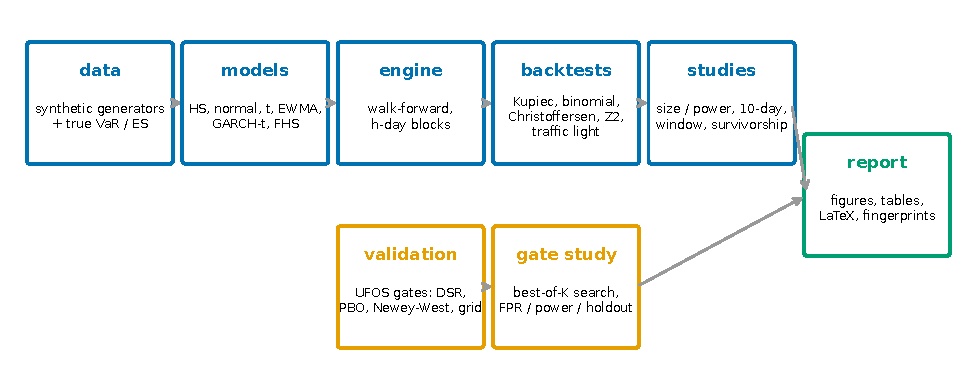
\includegraphics[width=\linewidth]{figures/fig12_architecture.pdf}
\caption{Risk Lab architecture. Blue: the market-risk pipeline from the synthetic data with known truth to the studies; orange: the re-implemented UFOS validation gates and their overfitting study; green: the report pipeline, which reads only saved, fingerprinted study results.}
\label{fig:fig12_architecture}
\end{figure}


\section*{Key results}
\begin{table}[H]
\centering
\footnotesize
\caption{Key results (synthetic data with known truth; Monte-Carlo rates $\pm$ se). Every number is read from the saved full runs in \texttt{studies/results/}.}
\label{tab:V1_key_results}
\setlength{\tabcolsep}{4pt}
\begin{tabular}{>{\raggedright\arraybackslash}p{1.9cm}>{\raggedright\arraybackslash}p{7.0cm}>{\raggedright\arraybackslash}p{3.6cm}>{\raggedright\arraybackslash}p{2.2cm}}
\toprule
Topic & Result & Value & Study \\
\midrule
Backtest size & Kupiec's exact size at T = 250 (nominal 5\,\%); exact binomial test & 9.48\,\%; 4.12\,\% & size / power \\
Estimation risk & Correct GARCH-t, 250-day window, T = 1000: Kupiec / Z2 rejection rate (exact Kupiec size 5.5\,\%) & 10.6 $\pm$ 1.0 / 17.7 $\pm$ 1.2\,\% & size / power \\
 & Same model, 500-day window: Kupiec; 1000 days: exceedance excess over the true VaR (pp) & 4.5 $\pm$ 0.7\,\%; +0.041 $\pm$ 0.007 & estimation window \\
Clustering & Static normal VaR on GARCH-t data, T = 1000: cc / Z2 rejection rate & 59.7 $\pm$ 1.6 / 64.7 $\pm$ 1.5\,\% & size / power \\
10-day VaR & $\sqrt{10}\times$ GARCH-t one-day VaR on iid $t_5$ data: relative bias & +8.6 $\pm$ 0.3\,\% & 10-day horizon \\
Survivorship & CAGR $\ge$ 10\,\% (hazard strength 1): survivors / counterfactual / full cohort; selection bias (pp) & 34.3 / 25.5 / 17.8\,\%; 8.8 $\pm$ 0.02 & survivorship \\
Gate study & UFOS statistical gates, standard: worst false-positive rate under noise; power at a true Sharpe of 1, $K$ = 64, 10 / 20 years & 0.5 $\pm$ 0.2\,\%; 13.1 $\pm$ 0.8 / 35.8 $\pm$ 1.1\,\% & gate overfitting \\
\bottomrule
\end{tabular}
\end{table}

In words: a one-year Kupiec backtest rejects a correct VaR almost twice as often as its nominal 5\,\%; a correctly
specified GARCH-$t$ with a 250-day estimation window still fails backtests about twice as often as it should,
which is estimation risk, and a window of 500 days or more removes most of it; static models miss volatility
clustering; $\sqrt{10}$ scaling of a fat-tailed one-day VaR overstates the 10-day VaR; survivors-only base rates
are strongly biased; and the UFOS validation gates stop searched noise rules but confirm a real Sharpe ratio of
1 only in a minority of cases. The figure below shows the estimation-window result.

\begin{figure}[H]
\centering
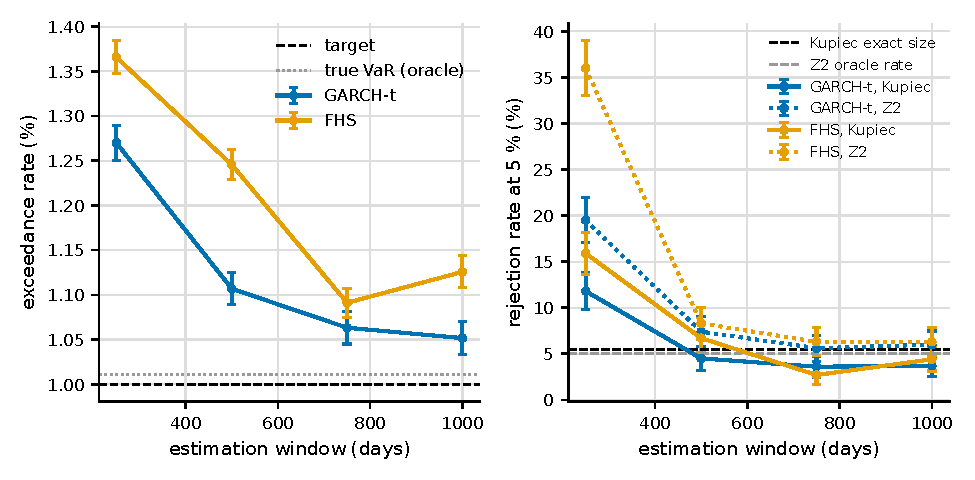
\includegraphics[width=\linewidth]{figures/fig3_estimation_window.pdf}
\caption{Estimation risk against the window length: correctly specified GARCH(1,1)-t and FHS on synthetic GARCH-t6 data, T = 1000 (the same forecast days for every window), M = 1000. Left: exceedance rate of the 99\,\% VaR, with the target and the oracle rate (the left axis does not start at 0); right: Kupiec and Z2 rejection rates with their reference sizes. Error bars $\pm 1.96$ se.}
\label{fig:fig3_estimation_window}
\end{figure}


\section*{How the results are made traceable}
\begin{itemize}
\item \textbf{Known truth:} every generator stores its true conditional parameters; the true VaR / ES are
  computed from them, so every model error and every test decision can be checked.
\item \textbf{Monte-Carlo uncertainty:} every rate carries its standard error; full runs use 1000 to 2000
  replications per setting.
\item \textbf{Fingerprints:} every saved full run records the sha256 of the code that produced it (the study
  script and the modules it imports), and the report build refuses results whose fingerprint does not match the
  current code.
\item \textbf{Reproducibility:} the same seed gives the same numbers within one numpy version; re-running all
  studies under a new package version gave identical results; figures and PDFs are byte-identical when rebuilt
  with the same tool versions.
\item \textbf{Tests and reviews:} 322 unit tests (closed forms, golden tables, smoke runs of every study); every
  version from v0.1 to v0.8 had an independent review whose findings were fixed in a follow-up round; a parity test checks the re-implemented
  validation gates against the platform's own code.
\end{itemize}

\section*{Reproduce}
From \texttt{UFOS.ai/RiskLab/} on Linux (verified with Python 3.10; hash-pinned dependencies):
\begin{verbatim}
python3 -m venv .venv && . .venv/bin/activate
python -m pip install --require-hashes -r requirements.lock
python -m unittest discover -s tests
python studies/var_backtest_power.py --mode smoke
python examples/quickstart.py
\end{verbatim}
The reports are built with \texttt{python report/build\_report.py --doc validation | overfitting | overview}
(needs \texttt{requirements-report.lock} and a TeX installation); the PDFs are not kept in the repository.

\section*{Limitations}
\begin{itemize}
\item Synthetic data only; the conclusions depend on the chosen generators and parameters, which are stated with
  every result. Real data would stay outside the repository.
\item One risk factor; no portfolios, no multivariate models, no Z1 / Z3 ES tests yet.
\item The gate study covers one rule family and part of the gates (G3, the cost and stress parts of G6 and G8 are
  out of scope).
\item The prose of the two detailed reports (validation report, gate study) is still open.
\end{itemize}

\section*{Since v0.7}
v0.7 adds interest rate risk in the banking book (IRRBB): Nelson--Siegel curves, banking-book instruments, the six
standardised shock scenarios with the post-shock floor, $\Delta$EVE / $\Delta$NII and the supervisory outlier
tests, with a study of a synthetic bank and its own report (\texttt{--doc irrbb}). v0.8 adds credit risk: a logistic
PD model with its validation tests, IFRS 9 expected credit loss and Basel IRB capital checked against the one-factor
loss distribution (\texttt{--doc credit}). v0.9 adds a free-cash-flow DCF and the reverse DCF (the growth a price
implies, compared with synthetic base rates), and a generic sensitivity toolkit -- tornado, two-way tables and
Sobol indices validated on the Ishigami function -- applied to the DCF, the IRRBB and the ECL models
(\texttt{--doc valuation}). The Risk Lab block ends with v0.9.

\end{document}
